% remember to set these at the start of each chapter
\chapter{Experiments and Discussion} 

%%%%%%%%%%%%%%%%%%
\section{Dataset}
The dataset is obtained from the study of \cite{Kosik2019}. It contains 90 specimen samples, each of which has an Ultrasound (US) image stack and a Photoacoustic (PAT) image stack. In the datadet, each specimen belongs to one of 14 types (class A - N) of cancer, actual cancer name is masked for simplicity. The distribution of classes is shown in Fig.\,\ref{class_graph}.  
\begin{figure}[h]
	\centering
	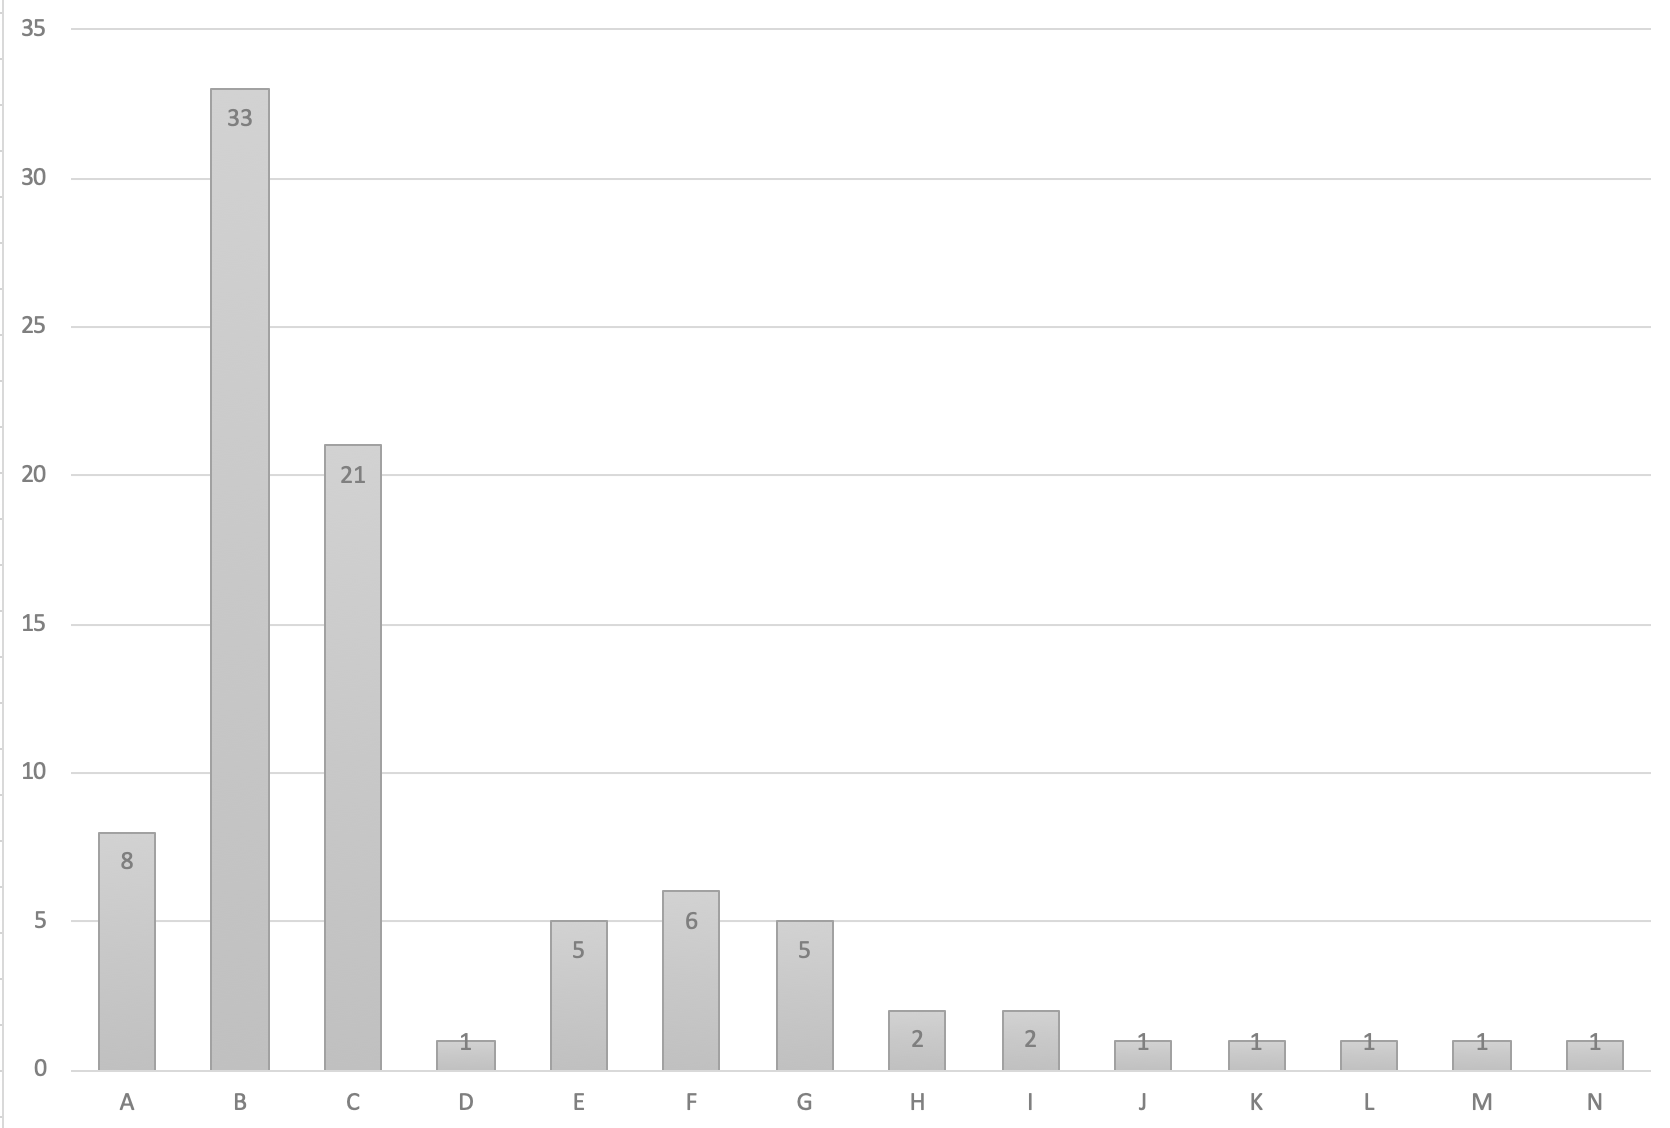
\includegraphics[width=0.8\textwidth]{Figs/class_graph.png}
    \caption{Cancer types}
    \label{class_graph}
\end{figure}
In this project, only class B and C are used. B has 33 samples and C has 21 samples. The other classes have too few samples to train a neural network on. 

In a vertical scan of a specimen, the centre few images usually have the most detail and thus have most information of the specimen which work best in classifying the specimen. An example of an image stack is shown in Fig.\,\ref{stack}. 

\begin{figure}[h]
	\centering
	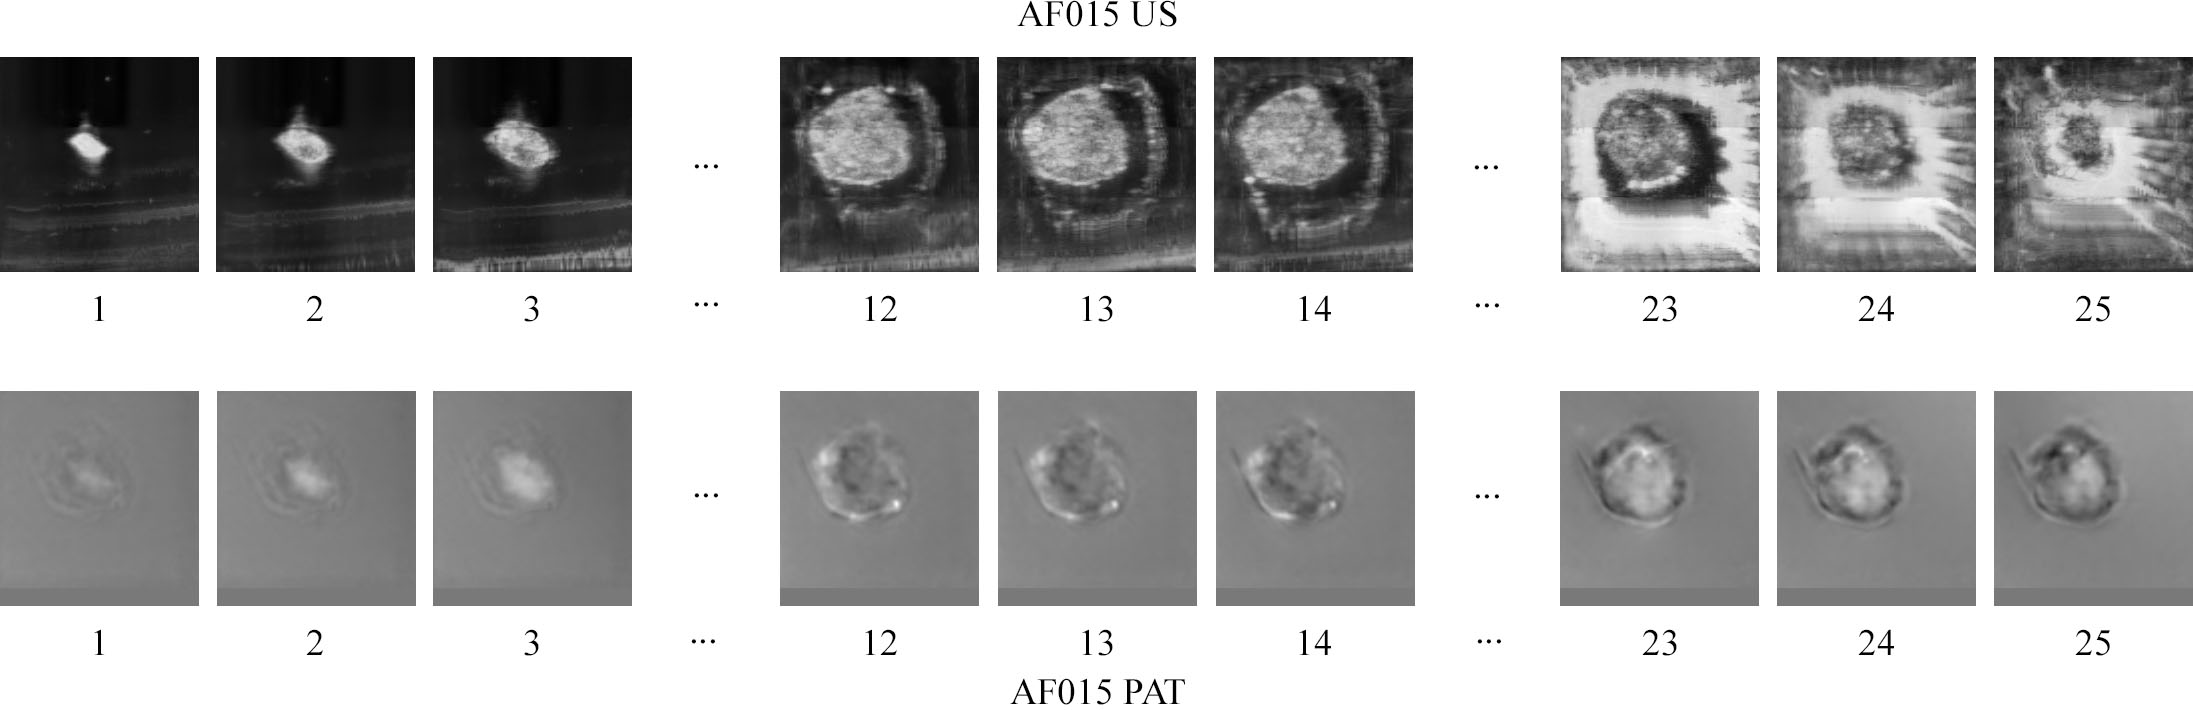
\includegraphics[width=\textwidth]{Figs/stack.jpg}
    \caption{US PAT stack example}
    \label{stack}
\end{figure}

We can see that the top and bottom few scans, for example 1, 2, 3, 23, 24, 25 in Fig.\,\ref{stack}, have very low quality and lack of detail about the internal texture. Scans close to centre of a specimen, such as 12, 13, 14, are larger in size and have the texture that classification may depend on. For each image stack, US and PAT, the centre 6 images are extracted to use for training and testing. There are in total 389 PAT images and 344 US images. Extracted PAT and US examples are shown in Fig.\,\ref{pat_us_example}.

\begin{figure}
\centering
\begin{subfigure}[b]{.24\linewidth}
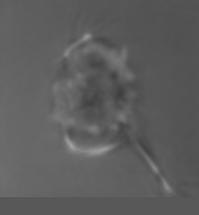
\includegraphics[width=\linewidth]{Figs/PAT014_18.jpg}
\caption{AF014 PAT}
\end{subfigure}
\begin{subfigure}[b]{.24\linewidth}
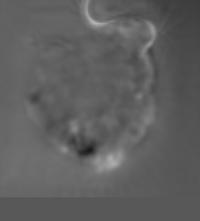
\includegraphics[width=\linewidth]{Figs/PAT023_23.jpg}
\caption{AF023 PAT}
\end{subfigure}
\begin{subfigure}[b]{.24\linewidth}
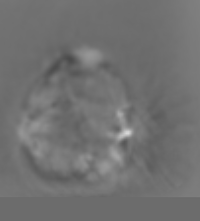
\includegraphics[width=\linewidth]{Figs/PAT36.png}
\caption{AF036 PAT}
\end{subfigure}
\begin{subfigure}[b]{.24\linewidth}
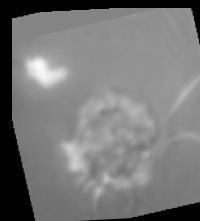
\includegraphics[width=\linewidth]{Figs/PAT055_11.jpg}
\caption{AF055 PAT}
\end{subfigure}

\begin{subfigure}[b]{.24\linewidth}
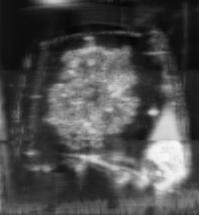
\includegraphics[width=\linewidth]{Figs/US14_18.jpg}
\caption{AF014 US}
\end{subfigure}
\begin{subfigure}[b]{.24\linewidth}
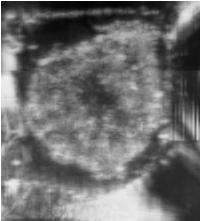
\includegraphics[width=\linewidth]{Figs/US23_23.jpg}
\caption{AF023 US}
\end{subfigure}
\begin{subfigure}[b]{.24\linewidth}
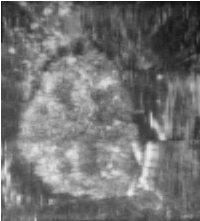
\includegraphics[width=\linewidth]{Figs/US36.png}
\caption{AF036 US}
\end{subfigure}
\begin{subfigure}[b]{.24\linewidth}
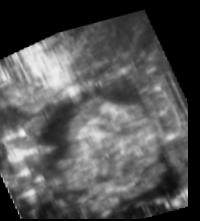
\includegraphics[width=\linewidth]{Figs/US55_13.jpg}
\caption{AF055 US}
\end{subfigure}
\caption{Extracted PAT and US examples}
\label{pat_us_example}
\end{figure}

\section{Data Partition and Augmentation}
The images are divided into a training set and a testing set by 0.8 ratio. No image from the same stack is separated into the training and the testing set. This is to ensure overfitting due to within-sample image similarities does not happen. Because the number of samples in class B and C is not balanced, K-fold data partitioning is done by using Stratified k-fold. The training set and the testing set contains approximately the same percentage of samples of each target class as the original dataset. Each of the five folds is used as a test set once and only once. Accuracy and $F_1$ score is averaged across five folds.

Machine learning requires large amounts of data. While our dataset is very small, data augmentation is used to artificially expand the number of samples (Fig.\,\ref{dataaug}) . Augmentation Scaling Factor is set to 5, meaning five images are created from one by Rotation, Cropping, Horizontal and Vertical Flip. Then, the images are resized to (192, 192).

\section{Training}
Adam \citep{adam} optimizer is used in all models to minimize the categorical cross-entropy across two classes. Adam is a replacement optimization algorithm for classic stochastic gradient descent. Adam can adaptively adjust the learning parameters based on the average first moment, as well as the average of the second moments of the gradients. The parameters of Adam optimizer is set to default. Training epoch is 50, all samples are passed to the network 50 times, with a batch size of 32. Best set of weights is saved. All parameters can be modified in YAML format for easier parameter fine tuning.


\section{Training Curves}
The learning process of a neural network can be investigated through training curves \citep{Anzanello2011}. Training and validation loss and accuracy are reported and ploted in Fig.\,\ref{fig:loss} and Fig.\,\ref{fig:acc}. VGG-IN is VGG model with ImageNet pre-trained weights loaded in the convolutional layers, Fully connected layer and classification layer are retrained.

\begin{figure}
\centering
\begin{subfigure}[b]{.45\linewidth}
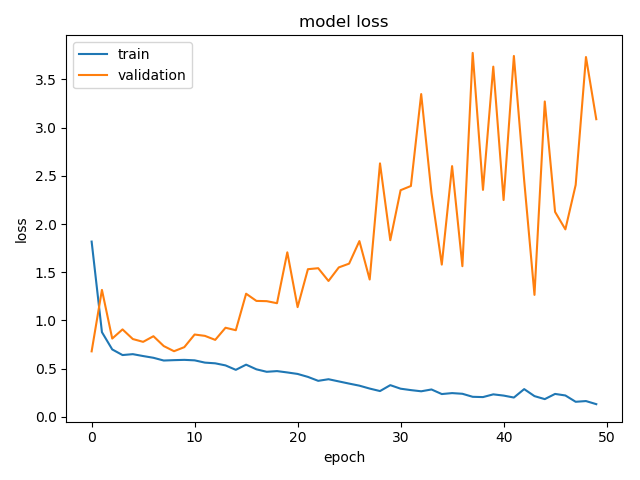
\includegraphics[width=\linewidth]{Figs/small_us_loss.jpg}
\caption{Small US}
\end{subfigure}
\begin{subfigure}[b]{.45\linewidth}
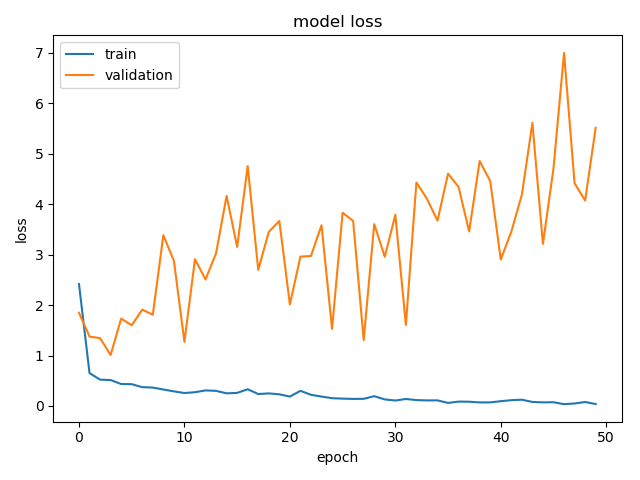
\includegraphics[width=\linewidth]{Figs/small_pat_loss.jpg}
\caption{Small PAT}
\end{subfigure}

\begin{subfigure}[b]{.45\linewidth}
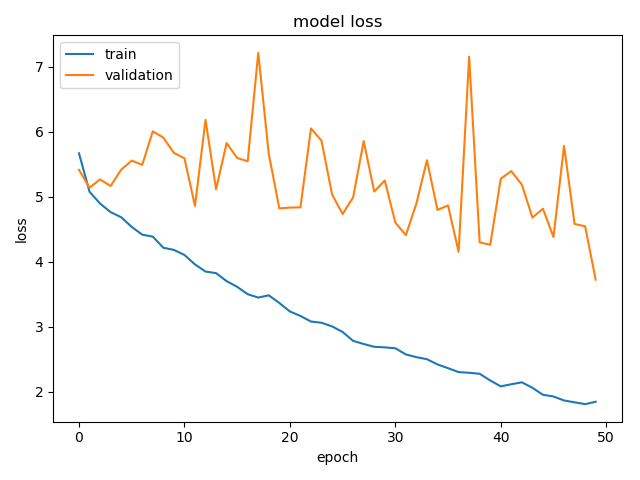
\includegraphics[width=\linewidth]{Figs/resnet_us_loss.jpg}
\caption{ResNet US}
\end{subfigure}
\begin{subfigure}[b]{.45\linewidth}
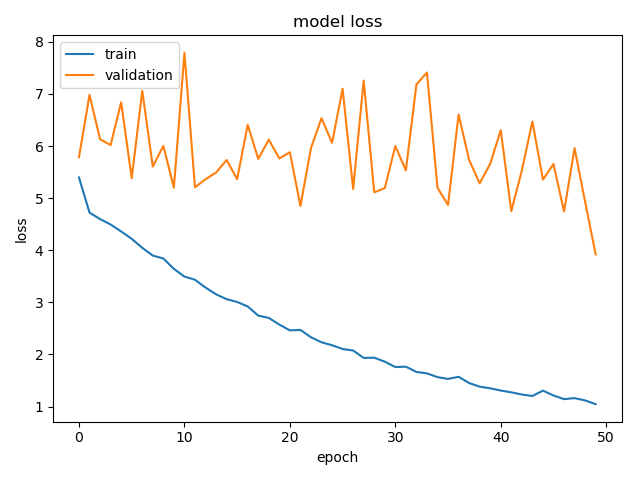
\includegraphics[width=\linewidth]{Figs/resnet_pat_loss.jpg}
\caption{ResNet PAT}
\end{subfigure}

\begin{subfigure}[b]{.45\linewidth}
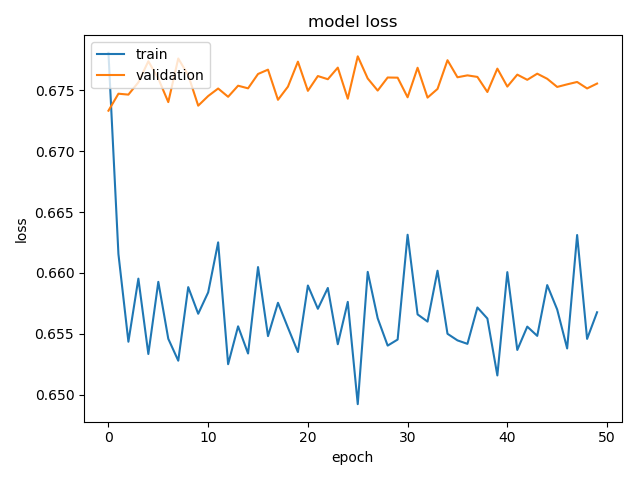
\includegraphics[width=\linewidth]{Figs/vgg_us_loss.jpg}
\caption{VGG US}
\end{subfigure}
\begin{subfigure}[b]{.45\linewidth}
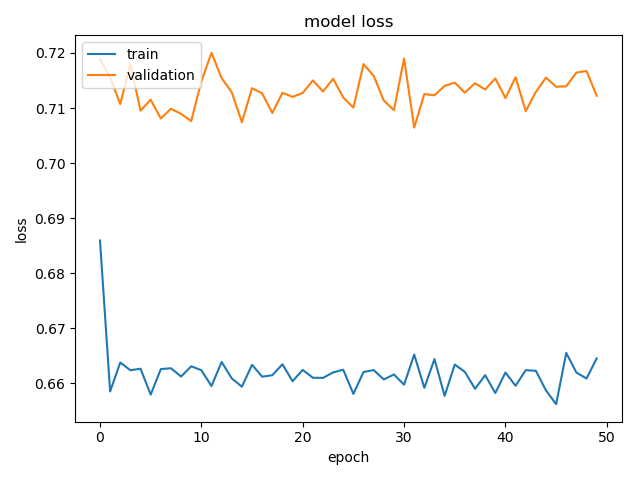
\includegraphics[width=\linewidth]{Figs/vgg_pat_loss.jpg}
\caption{VGG PAT}
\end{subfigure}

\begin{subfigure}[b]{.45\linewidth}
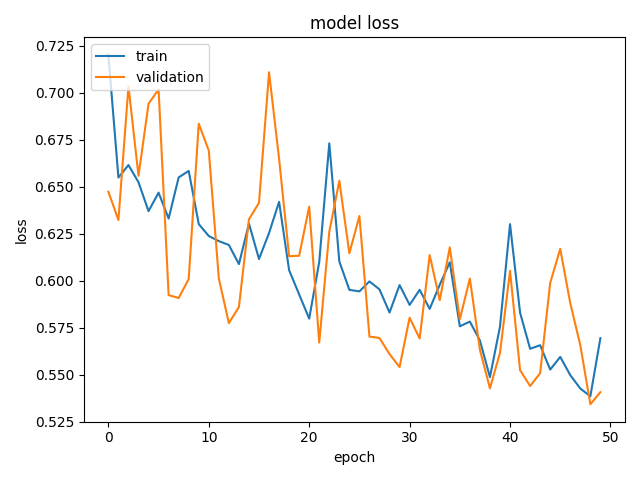
\includegraphics[width=\linewidth]{Figs/vgg_in_us_loss.jpg}
\caption{VGG-IN US}
\end{subfigure}
\begin{subfigure}[b]{.45\linewidth}
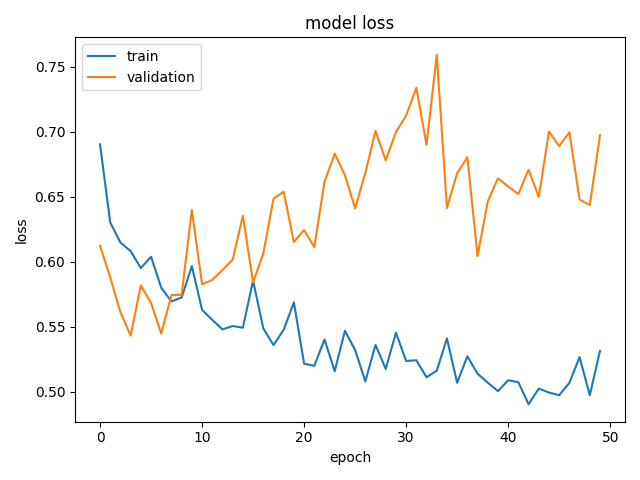
\includegraphics[width=\linewidth]{Figs/vgg_in_pat_loss.jpg}
\caption{VGG-IN PAT}
\end{subfigure}
\caption{Model loss}
\label{fig:loss}
\end{figure}

\begin{figure}
\centering
\begin{subfigure}[b]{.45\linewidth}
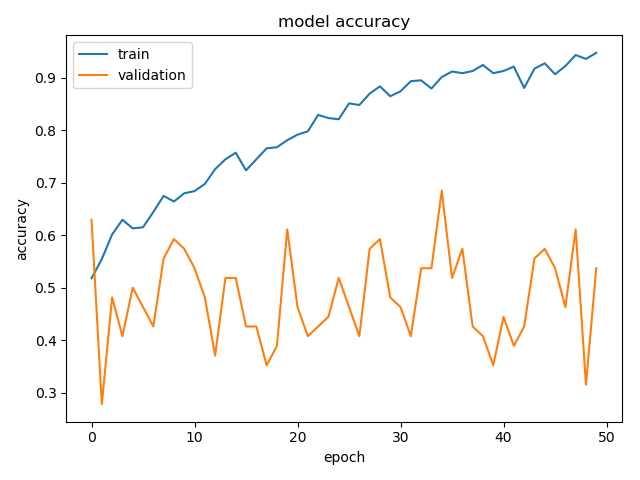
\includegraphics[width=\linewidth]{Figs/small_us_acc.jpg}
\caption{Small US}
\end{subfigure}
\begin{subfigure}[b]{.45\linewidth}
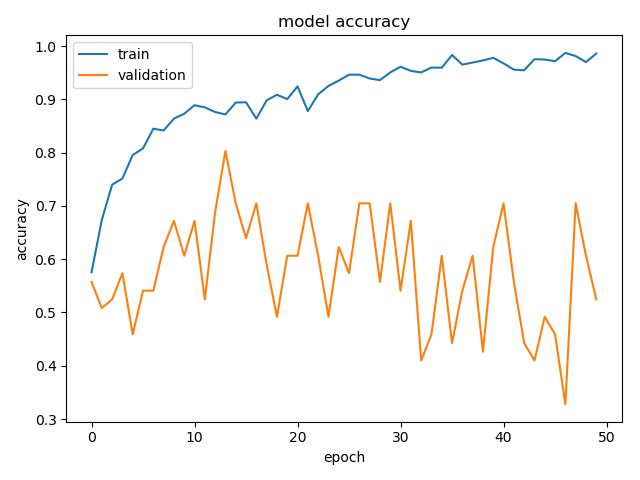
\includegraphics[width=\linewidth]{Figs/small_pat_acc.jpg}
\caption{Small PAT}
\end{subfigure}

\begin{subfigure}[b]{.45\linewidth}
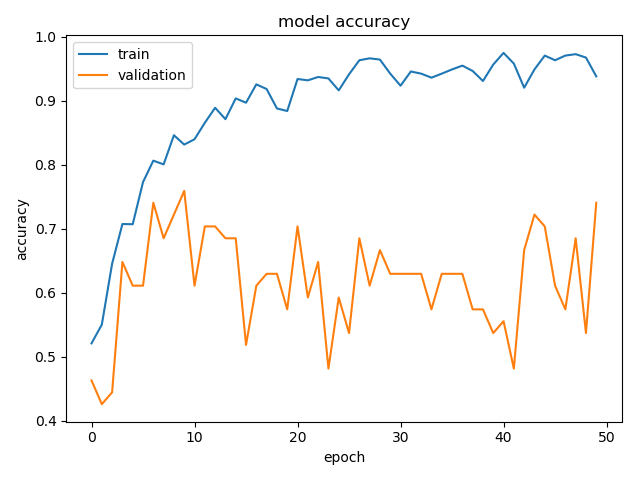
\includegraphics[width=\linewidth]{Figs/resnet_us_acc.jpg}
\caption{ResNet US}
\end{subfigure}
\begin{subfigure}[b]{.45\linewidth}
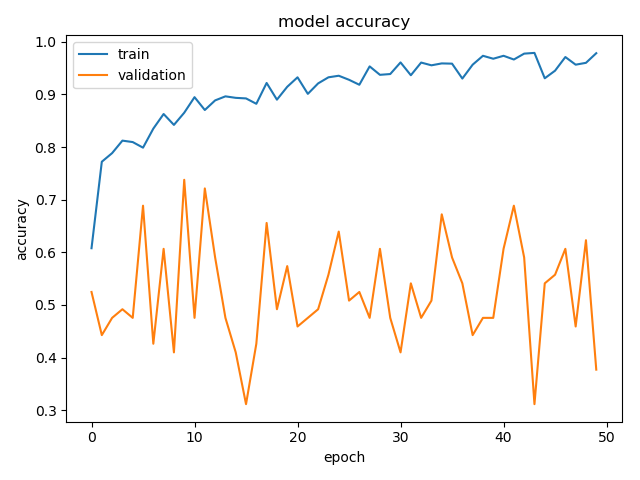
\includegraphics[width=\linewidth]{Figs/resnet_pat_acc.jpg}
\caption{ResNet PAT}
\end{subfigure}

\begin{subfigure}[b]{.45\linewidth}
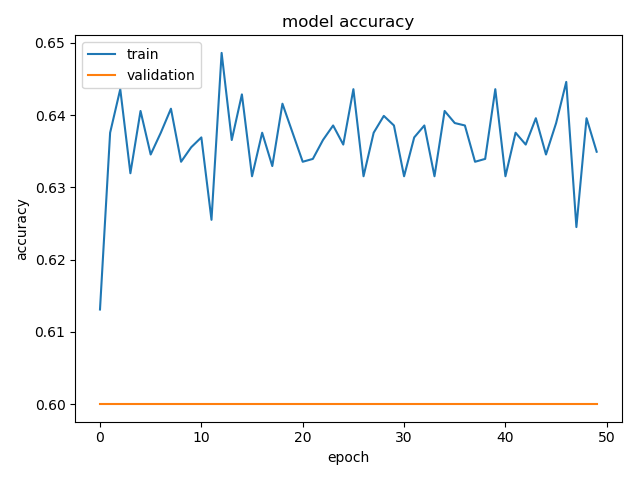
\includegraphics[width=\linewidth]{Figs/vgg_us_acc.jpg}
\caption{VGG US}
\end{subfigure}
\begin{subfigure}[b]{.45\linewidth}
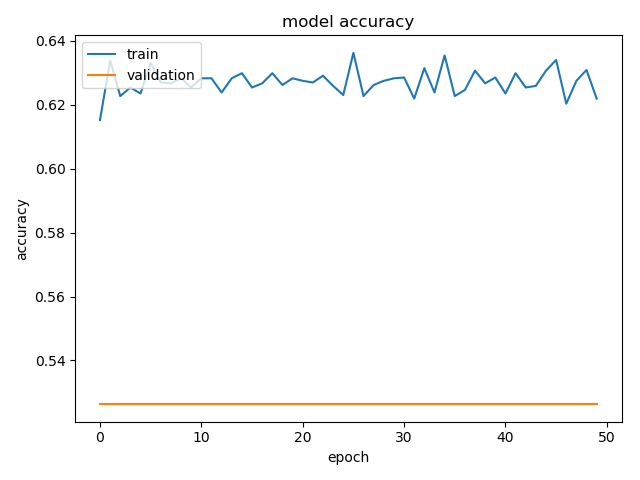
\includegraphics[width=\linewidth]{Figs/vgg_pat_acc.jpg}
\caption{VGG PAT}
\end{subfigure}

\begin{subfigure}[b]{.45\linewidth}
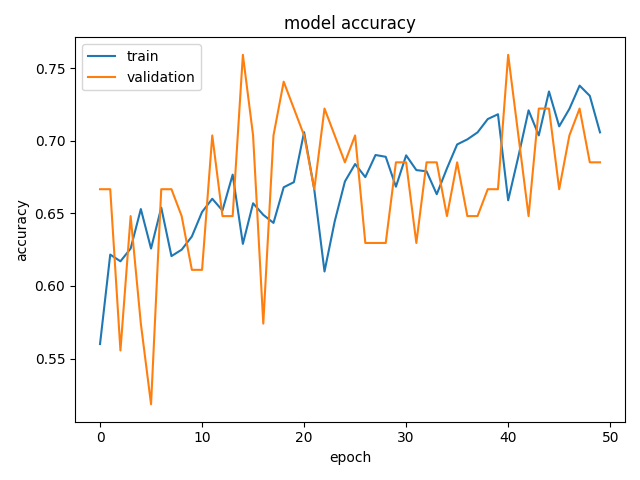
\includegraphics[width=\linewidth]{Figs/vgg_in_us_acc.jpg}
\caption{VGG-IN US}
\end{subfigure}
\begin{subfigure}[b]{.45\linewidth}
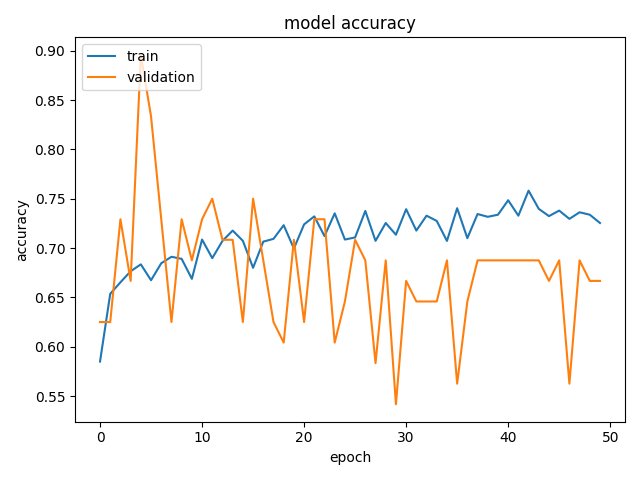
\includegraphics[width=\linewidth]{Figs/vgg_in_pat_acc.jpg}
\caption{VGG-IN PAT}
\end{subfigure}
\caption{Model accuracy}
\label{fig:acc}
\end{figure}

The validation loss and accuracy are very noise, and do not have much improvement. Note that there is a large gap between training and validation curves. This indicates that the training dataset is unrepresentative, which means the training dataset does not provide sufficient information to learn the problem. We have too few examples in the dataset. From the noisy validation curves, we can conclude that the validation dataset is also unrepresentative. A  unrepresentative validation set means that it does not provide sufficient information to evaluate the ability of the model to generalize. This could occur when the validation dataset has too few examples.

\section{Accuracy and $F_1$ score}
The $F_1$ score (also F-score) is a measure of a test's accuracy \citep{powers2011evaluation}. It considers both the precision $p$ and the recall $r$ of the test to compute the score: $p$ is the number of correct positive results divided by the number of all positive results returned by the classifier, and $r$ is the number of correct positive results divided by the number of all relevant samples (all samples that should have been identified as positive). The $F_1$ score is the harmonic average of the precision and recall, where an $F_1$ score reaches its best value at 1 (perfect precision and recall) and worst at 0.
Formally: $$F_1 score = 2 \cdot \frac{precision \cdot recall}{precision + recall}$$
Presition: $$p = \frac{TP}{TP + FP}$$
Recall: $$r = \frac{TP}{TP + FN}$$
\noindent True Positives (TP): Samples which we predicted belong to a class, and they are indeed in the class.

\noindent True Negatives (TN): Samples which we predicted not belong to a class, and they are indeed not in that class.

\noindent False Positives (FP): We predicted in a class, but they are actually not.

\noindent False Negatives (FN): We predicted not in a class, but they are actually in.

\begin{table}[h]
\centering
\begin{tabular}{ |p{4cm}||p{3cm}|p{3cm}|p{3cm}|  }
 \hline
 Model       & Accuracy & Class B $F_1$ score & Class C $F_1$ score\\
 \hline
 \hline
 Small  US   & 0.66  & 0.77 &  0.23\\
 ResNet US   & 0.75  & 0.82 &  0.55\\
 VGG US      & 0.61  & 0.76 &  0\\
 VGG-ImageNet US & 0.65 & 0.77 & 0.22 \\
\hline
 Small PAT   & 0.71  & 0.79 &  0.50\\
 ResNet PAT  & 0.76  & 0.83 &  0.57\\
 VGG PAT     & 0.61  & 0.76 &  0\\
 VGG-ImageNet PAT & 0.78 & 0.84 & 0.54 \\
 \hline
\end{tabular}
\caption{Model accuracy and $F_1$ score}
\label{acctable}
\end{table}

\section{Discussion}
Benefits from shortcut connections, even though ResNet model is deep, it could converge reasonable well. The decrease of training loss indicated that ResNet was training from the training set. On the other hand, the convergence of training loss of a deep CNN model is very poor. VGG model was too deep to train. Trying to address this problem, in VGG-IN model, ImageNet pre-trained weights were loaded. However, the training result was still not satisfactory. All models performed poorly on our dataset comparing to their original benchmark. To verify that the models were correctly implemented, they were trained on other datasets. Results are shown in Appendix \ref{appendixB}. 

Medical images are naturally difficult to acquire. By machine learning standard, which often requires thousands or even hundreds of thousands samples, our dataset is considered extremely small. In addition, the US and PAT scans are very noisy and have lots of artifacts. The low quality of images makes it more challenging to pick up details for learning. Examples are shown in Fig.\,\ref{stack} and Fig.\,\ref{pat_us_example}. With additional data come to hand, we hope to see an improvement on the models' performance.

\section{Experiments with other datasets}

Due to the poor performance in experiments with our dataset, to verify that the neural network models are correctly implemented, the models are trained on other classification datasets \citep{Janowczyk2016} and \citep{catdog}.

From the results, we can see that neural network models benefit from large amounts of data. The loss is decreasing and accuracy is increasing for both IDC Breast Cancer dataset and cat\&dog dataset. Accuracy and $F_1$ score is reported in Table \ref{acctable2}.


\begin{figure}
\centering
\begin{subfigure}[b]{.2\linewidth}
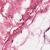
\includegraphics[width=\linewidth]{Figs/8864_idx5_x1251_y1651_class0.png}
\end{subfigure}
\begin{subfigure}[b]{.2\linewidth}
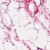
\includegraphics[width=\linewidth]{Figs/8864_idx5_x1201_y1801_class0.png}
\end{subfigure}
\begin{subfigure}[b]{.2\linewidth}
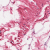
\includegraphics[width=\linewidth]{Figs/8864_idx5_x1201_y1701_class0.png}
\end{subfigure}
\begin{subfigure}[b]{.2\linewidth}
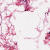
\includegraphics[width=\linewidth]{Figs/8864_idx5_x1151_y1701_class0.png}
\end{subfigure}

\begin{subfigure}[b]{.2\linewidth}
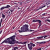
\includegraphics[width=\linewidth]{Figs/8864_idx5_x1851_y2251_class1.png}
\end{subfigure}
\begin{subfigure}[b]{.2\linewidth}
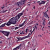
\includegraphics[width=\linewidth]{Figs/8864_idx5_x1801_y2701_class1.png}
\end{subfigure}
\begin{subfigure}[b]{.2\linewidth}
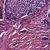
\includegraphics[width=\linewidth]{Figs/8864_idx5_x1801_y2651_class1.png}
\end{subfigure}
\begin{subfigure}[b]{.2\linewidth}
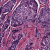
\includegraphics[width=\linewidth]{Figs/8864_idx5_x1801_y2551_class1.png}
\end{subfigure}
\caption{IDC Breast Cancer Dataset: class0 \& class1}
\label{IDC}
\end{figure}


\begin{figure}
\centering
\begin{subfigure}[b]{.2\linewidth}
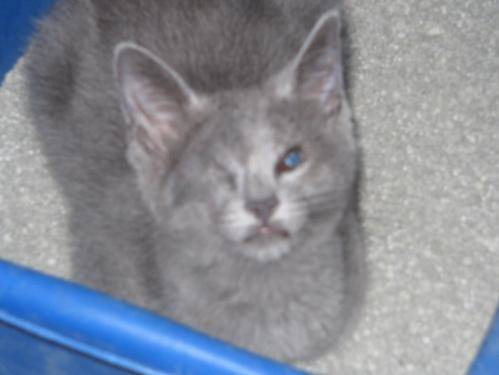
\includegraphics[width=\linewidth]{Figs/cat450.jpg}
\end{subfigure}
\begin{subfigure}[b]{.2\linewidth}
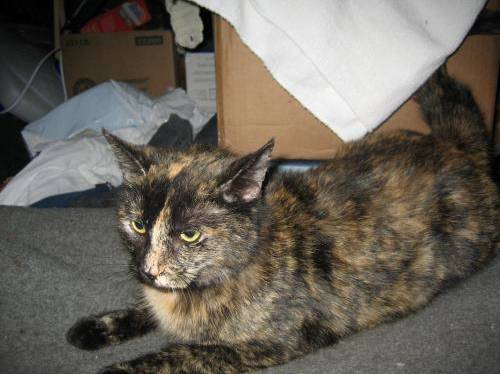
\includegraphics[width=\linewidth]{Figs/cat1921.jpg}
\end{subfigure}
\begin{subfigure}[b]{.2\linewidth}
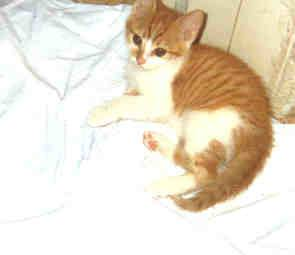
\includegraphics[width=\linewidth]{Figs/cat1412.jpg}
\end{subfigure}
\begin{subfigure}[b]{.2\linewidth}
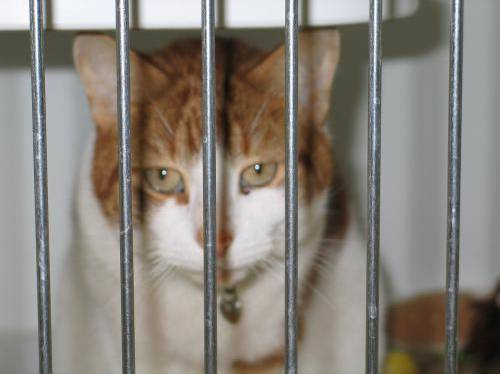
\includegraphics[width=\linewidth]{Figs/cat1168.jpg}
\end{subfigure}

\begin{subfigure}[b]{.2\linewidth}
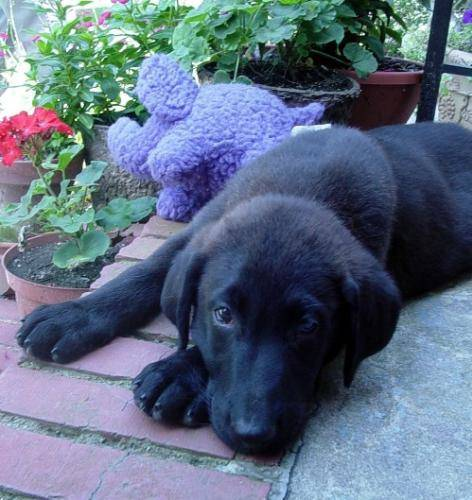
\includegraphics[width=\linewidth]{Figs/dog876.jpg}
\end{subfigure}
\begin{subfigure}[b]{.2\linewidth}
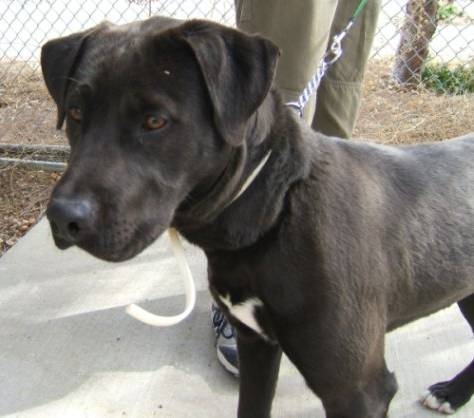
\includegraphics[width=\linewidth]{Figs/dog508.jpg}
\end{subfigure}
\begin{subfigure}[b]{.2\linewidth}
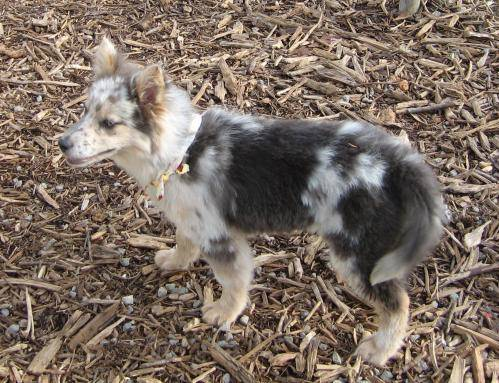
\includegraphics[width=\linewidth]{Figs/dog4133.jpg}
\end{subfigure}
\begin{subfigure}[b]{.2\linewidth}
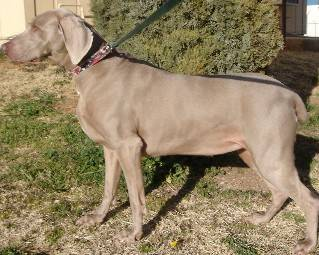
\includegraphics[width=\linewidth]{Figs/dog1178.jpg}
\end{subfigure}
\caption{Cats \& Dogs Dataset}
\label{catdog}
\end{figure}


\begin{figure}
\centering
\begin{subfigure}[b]{.45\linewidth}
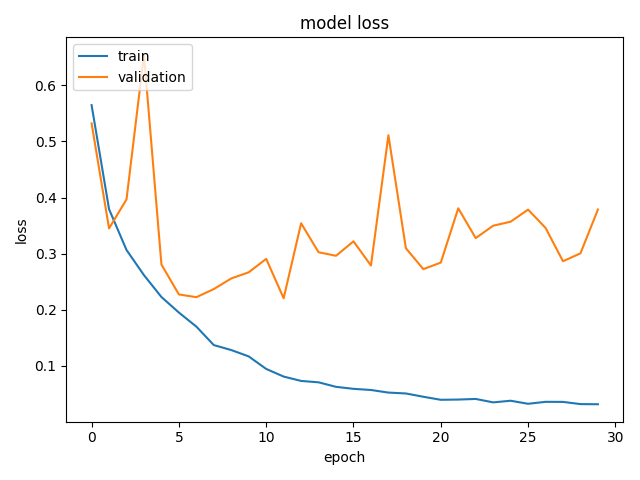
\includegraphics[width=\linewidth]{Figs/small_catdog_loss.jpg}
\caption{Small CatDog}
\end{subfigure}
\begin{subfigure}[b]{.45\linewidth}
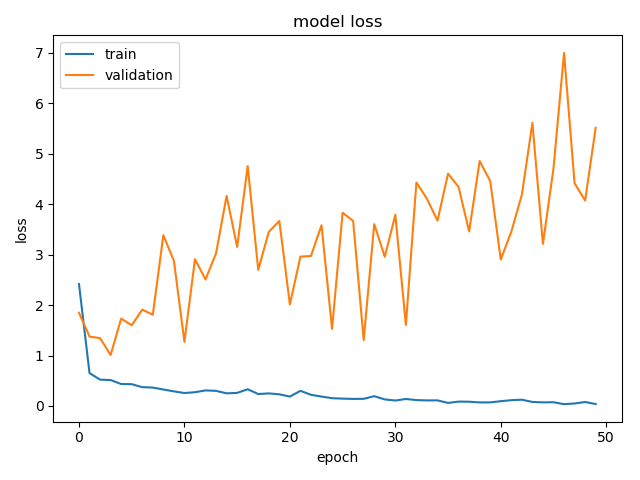
\includegraphics[width=\linewidth]{Figs/small_pat_loss.jpg}
\caption{Small PAT}
\end{subfigure}

\begin{subfigure}[b]{.45\linewidth}
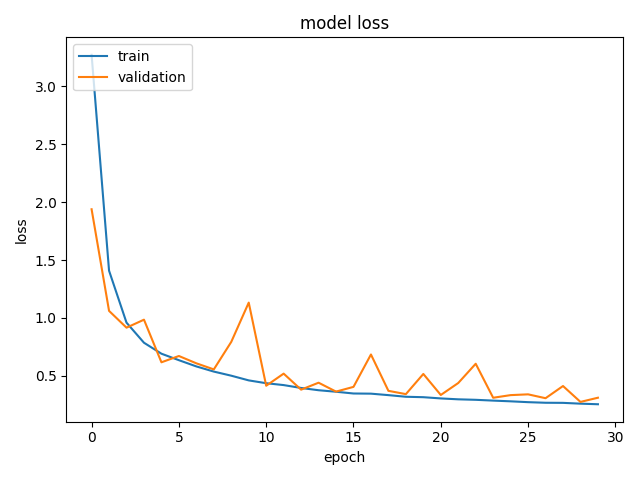
\includegraphics[width=\linewidth]{Figs/resnet_catdog_loss.jpg}
\caption{ResNet CatDog}
\end{subfigure}
\begin{subfigure}[b]{.45\linewidth}
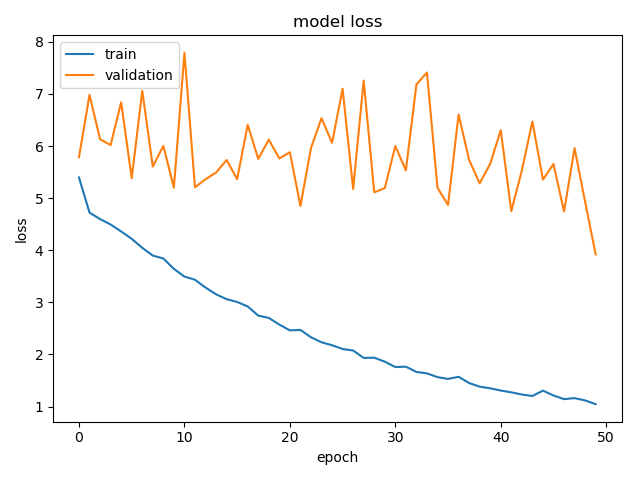
\includegraphics[width=\linewidth]{Figs/resnet_pat_loss.jpg}
\caption{ResNet PAT}
\end{subfigure}

\begin{subfigure}[b]{.45\linewidth}
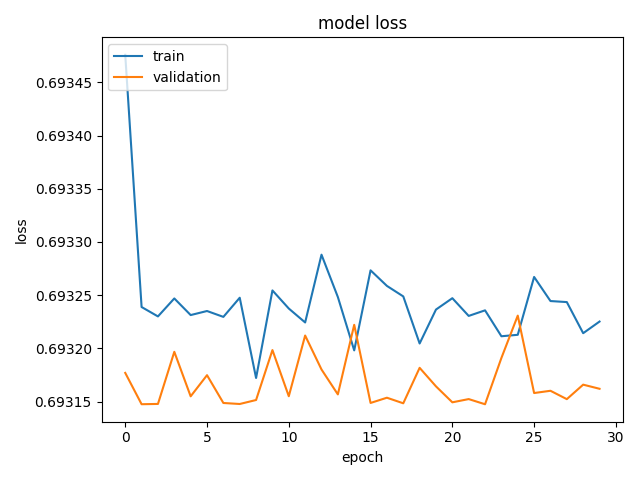
\includegraphics[width=\linewidth]{Figs/vgg_catdog_loss.jpg}
\caption{VGG CatDog}
\end{subfigure}
\begin{subfigure}[b]{.45\linewidth}
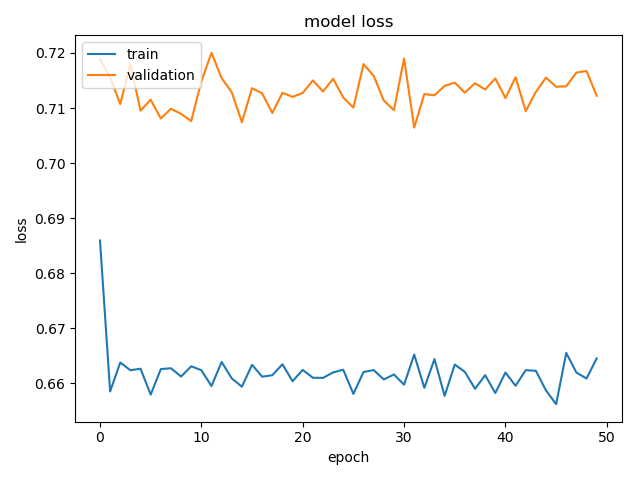
\includegraphics[width=\linewidth]{Figs/vgg_pat_loss.jpg}
\caption{VGG PAT}
\end{subfigure}

\begin{subfigure}[b]{.45\linewidth}
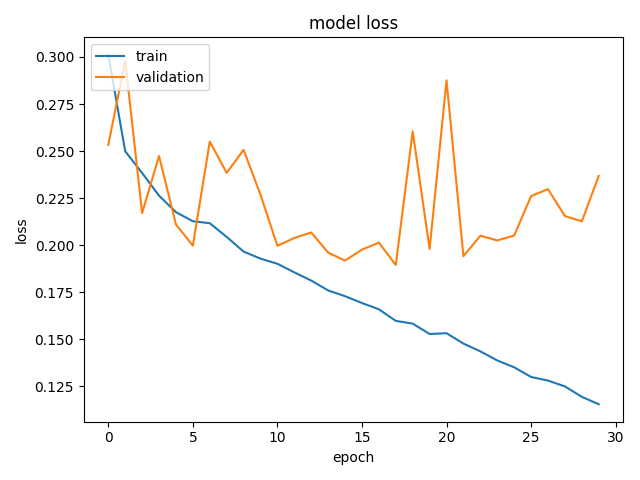
\includegraphics[width=\linewidth]{Figs/vgg_in_catdog_loss.jpg}
\caption{VGG-IN CatDog}
\end{subfigure}
\begin{subfigure}[b]{.45\linewidth}
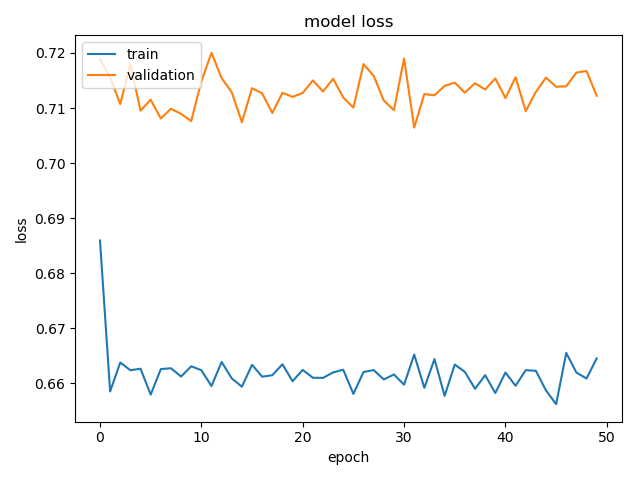
\includegraphics[width=\linewidth]{Figs/vgg_pat_loss.jpg}
\caption{VGG-IN PAT}
\end{subfigure}
\caption{Model loss}
\label{fig:loss2}
\end{figure}

\begin{figure}
\centering
\begin{subfigure}[b]{.45\linewidth}
\includegraphics[width=\linewidth]{Figs/small_catdog_acc.jpg}
\caption{Small CatDog}
\end{subfigure}
\begin{subfigure}[b]{.45\linewidth}
\includegraphics[width=\linewidth]{Figs/small_pat_acc.jpg}
\caption{Small PAT}
\end{subfigure}

\begin{subfigure}[b]{.45\linewidth}
\includegraphics[width=\linewidth]{Figs/resnet_catdog_acc.jpg}
\caption{ResNet CatDog}
\end{subfigure}
\begin{subfigure}[b]{.45\linewidth}
\includegraphics[width=\linewidth]{Figs/resnet_pat_acc.jpg}
\caption{ResNet PAT}
\end{subfigure}

\begin{subfigure}[b]{.45\linewidth}
\includegraphics[width=\linewidth]{Figs/vgg_catdog_acc.jpg}
\caption{VGG CatDog}
\end{subfigure}
\begin{subfigure}[b]{.45\linewidth}
\includegraphics[width=\linewidth]{Figs/vgg_pat_acc.jpg}
\caption{VGG PAT}
\end{subfigure}

\begin{subfigure}[b]{.45\linewidth}
\includegraphics[width=\linewidth]{Figs/vgg_in_catdog_acc.jpg}
\caption{VGG-IN CatDog}
\end{subfigure}
\begin{subfigure}[b]{.45\linewidth}
\includegraphics[width=\linewidth]{Figs/vgg_pat_acc.jpg}
\caption{VGG-IN PAT}
\end{subfigure}
\caption{Model accuracy}
\label{fig:acc2}
\end{figure}

\begin{table}
\centering
\begin{tabular}{ |p{3cm}||p{3cm}|p{3cm}|p{3cm}|  }
 \hline
 Model       & Accuracy & Class 0 $F_1$ score & Class 1 $F_1$ score\\
 \hline
 \hline
 Small Breast   & 0.90  & 0.94 &  0.78\\
 ResNet Breast  & 0.91  & 0.94 &  0.80\\
 VGG Breast      & 0.77  & 0.87 &  0\\
 VGG-IN breast & 0 & 0 & 0 \\
 \hline
 Small CatDog   & 0.93  & 0.93 &  0.93\\
 ResNet CatDog  & 0.93  & 0.93 &  0.93\\
 VGG CatDog      & 0.50  & 0.67 &  0\\
 VGG-IN CatDog & 0.92 & 0.92 & 0.92 \\
  \hline
\end{tabular}
\caption{Model accuracy and $F_1$ score}
\label{acctable2}
\end{table}
